\begin{frame}
	\frametitle{Redes neurais residuais (ResNets)}
	
	\only<1>{
		\par Redes neurais profundas podem sofrer com desaparecimento ou explosão do gradiente. A solução é reproduzir o comportamento de redes neurais mais rasas usando conexões de salto. Essa é ideia das redes neurais residuais.
	}
	
	\only<2>{
		\begin{columns}
			\column{.5\linewidth}
				\begin{figure}[H]
					\centering
					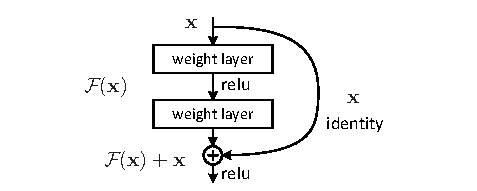
\includegraphics[width=1\linewidth]{../monography/images/residualBlock}
					\label{fig:residualblock}
				\end{figure}
			\column{.5\linewidth}
				\par Segundo \cite{DBLP:journals/corr/HeZRS15} a ideia-chave por trás das \textit{ResNets} é a inclusão de conexões de salto como ilustrado na  figura ao lado, também conhecidas como mapeamentos de identidade.
				
				\par Bloco Residual: $x$ contorna as camada intermediárias $F(x)$ via uma função identidade somando-se a $F(x)$ ao final do bloco.
		\end{columns}
	}
	
	\only<3>{
		\par Obtenção do resíduo: $x$ um vetor de entrada na rede, $I(\cdot)$ é uma função identidade cujo valor é diretamente somado $\oplus$ com o resultado produzido pelas várias camadas representadas por $f(\cdot)$, $h$ é um vetor representando um estado intermediário de uma rede neural.
		\begin{figure}[h]
			\centering
			\begin{tikzpicture}[node distance=3cm, every edge/.style={draw=black,->}]
	% Nodes
	\node[draw, rectangle, fill=blue] (x) {$x$};
	\node[draw, rectangle, above right=-.6cm and 1cm of x] (function) {$r = f(x)$};
	\node[draw, rectangle, above right=1cm and -1.1cm of function] (identi) {$I(x)$};
	\node[draw, circle, above right=-.5cm and 4cm of x] (plus) {$+$};
	\node[draw, rectangle, above right=-.6cm and 1.5cm of plus, fill=gray] (hidden) {$h$};
	
	% Arrows
	\draw (x) edge (function);
	\draw (function) edge (plus);
	\draw (plus) edge (hidden);
	
	
	\draw [->,in=180,out=90](x) edge (identi);
	\draw [->,in=90,out=0] (identi) edge (plus);
	

	% Labels
	\node[above of=identi, yshift=-2.4cm] {Identidade};
	\node[above of=x, yshift=-4cm] {Entrada};
	\node[above of=hidden, yshift=-4cm, xshift=0cm] {Estado intermediário};
\end{tikzpicture}
			\label{fig:residuo}
		\end{figure}
	}
\end{frame}